\subsection{膜展開部(および膜上デバイス制御部)}

膜展開部周辺の1Uサイズの中の機器は,正確には「膜展開部」と「膜上デバイス制御部(MDC)」の2つのサブシステムに分割される.さらに,両システムにまたがって配置される膜上のアドバンストミッション機器がある.それぞれについて以下に述べる.

\subsubsection{展開膜開発(サカセアドテック・古谷・坂本)}

下図に概要を示すような膜展開部を開発した.サカセアドテック社,古谷研メンバー,坂本研メンバーで設計・評価を行い,製造はほぼすべてをサカセアドテック社が担った.ほぼ全体が新規開発であり,たいへんに挑戦的な開発だったが,フライトに供することが可能なミッションペイロードを開発完了できた.
\begin{figure}[H]
	\centering
	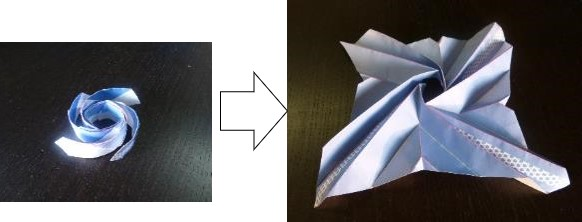
\includegraphics[width=.5\textwidth]{03/fig/3-9-3-1-4.jpg}
	\caption{多機能展開膜のたたみ方を示す折り紙モデル}
	\label{fig3-9-3-1-4}
\end{figure}
\begin{figure}[H]
	\centering
	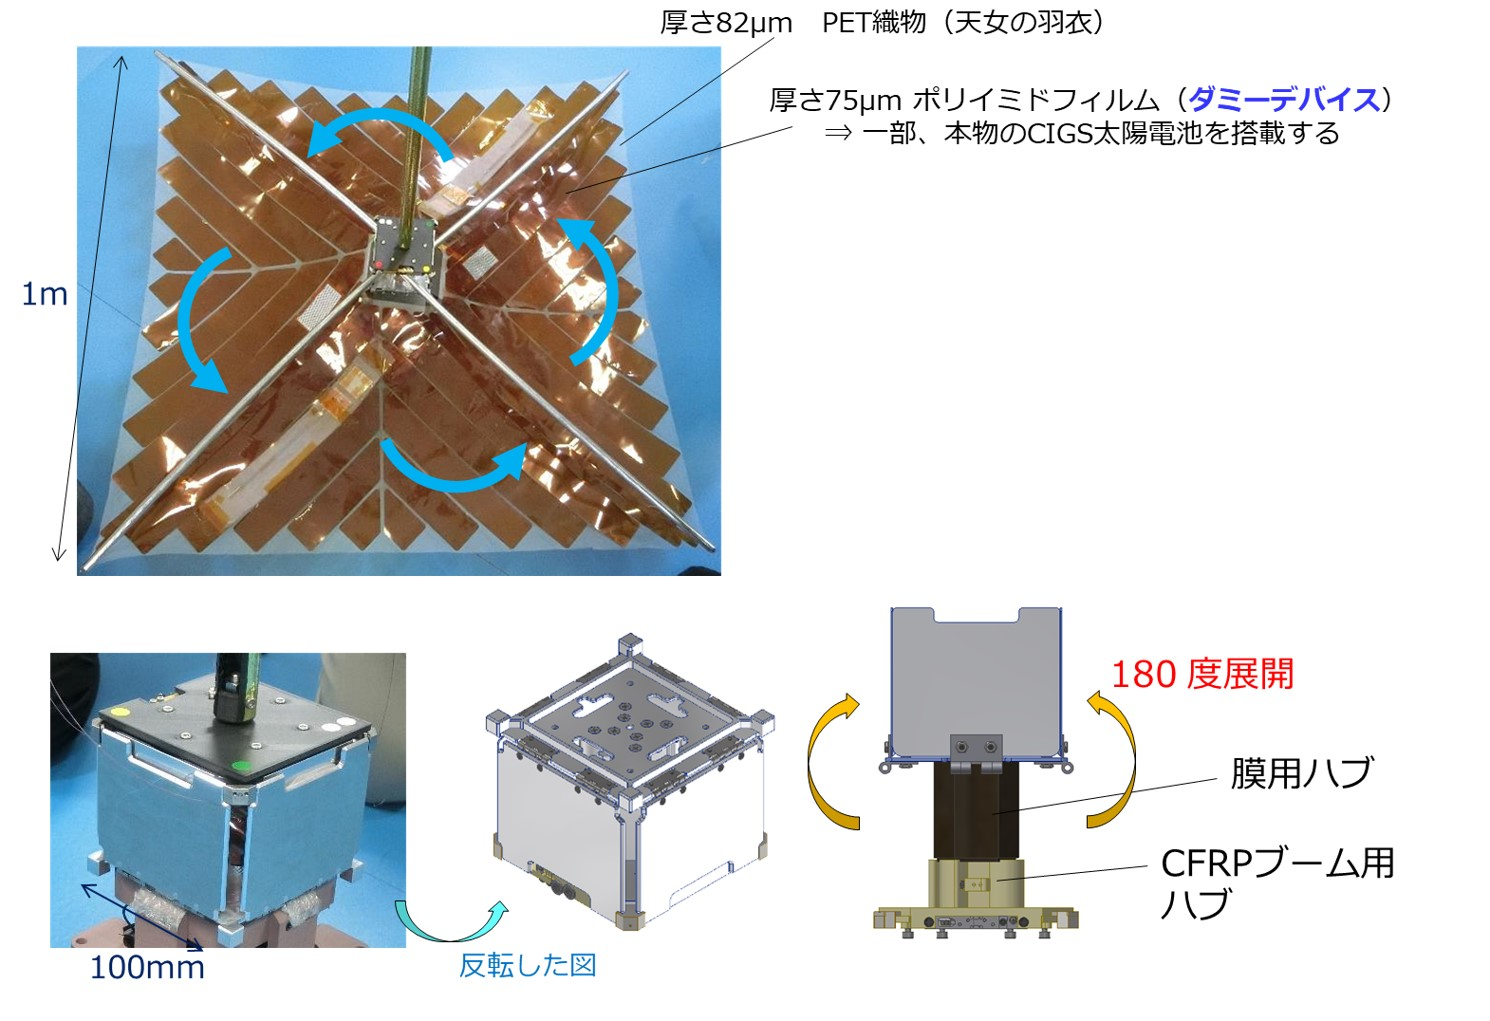
\includegraphics[width=.8\textwidth]{03/fig/3-9-3-1-1.jpg}
	\caption{EMの膜展開部:ダミーデバイスとしてカプトンを使用}
	\label{fig3-9-3-1-1}
\end{figure}
\begin{figure}[H]
	\centering
	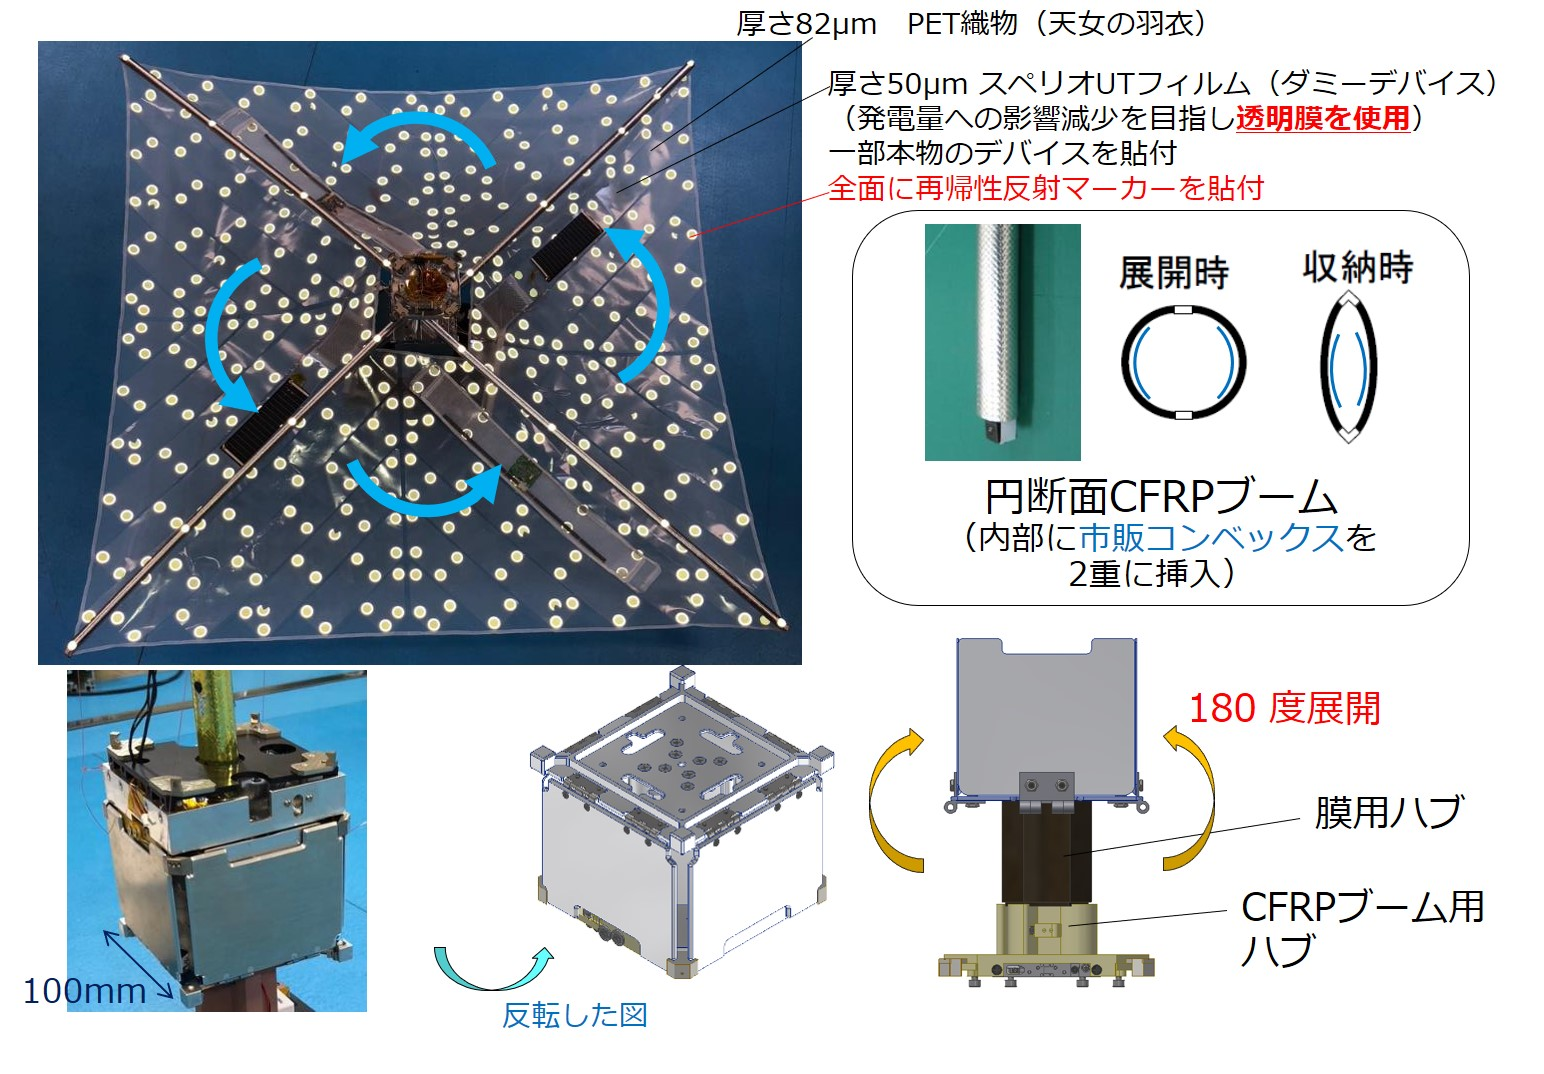
\includegraphics[width=.8\textwidth]{03/fig/3-9-3-1-2.jpg}
	\caption{FMの膜展開部:ダミーデバイスとしてスペリオUTを使用}
	\label{fig3-9-3-1-2}
\end{figure}
\begin{figure}[H]
	\centering
	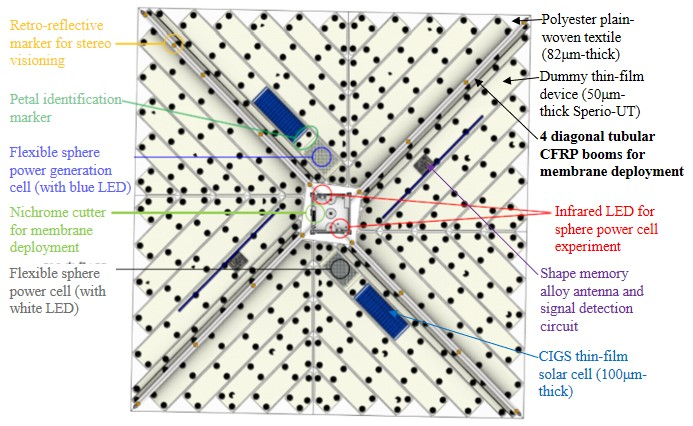
\includegraphics[width=.8\textwidth]{03/fig/3-9-3-1-3.jpg}
	\caption{FM膜上に貼付した各種デバイス}
	\label{fig3-9-3-1-3}
\end{figure}
特に大きな特徴として下記3つがある.
\begin{itemize}
	\item 平織布をベース膜として用いている.この織物の伸縮性により,膜上デバイスの厚さを吸収してコンパクトな収納を可能とし,さらに折り目が高い剛性を持たず展開を阻害しない膜とした.
	\item 円筒形のCFRPブームの中に2本のステンレス製コンベックステープを向かい合わせに挿入した「ハイブリッドブーム」を新たに提案し搭載した(図\ref{fig3-9-3-1-2}).ステンレス製コンベックステープは長期収納後でも展開力が減じにくいが,展開後形状を保つ剛性は持ちにくい.一方,円筒型CFRPブームは,展開力は長期収納の影響で減じやすいが,円形断面にひとたび展開すれば,形状を維持する剛性を提供できる.
	\item 小さな容積の中に,4つのウォールが同期して展開する機構を収めた.テグスの溶断によりこの機構が動作する.テグス溶断の仕組みについては別項にて後述する.
\end{itemize}

この膜展開部の開発経緯や,設計については,サカセアドテック社が膜展開部についての記述を担当した下記の公開文書に極めて詳細に記録されているため,ここでは割愛する.
\begin{itemize}
	\item 平成28年度 宇宙航空科学技術推進委託費「革新的宇宙科学を切り拓く先進展開構造の研究・開発拠点形成」委託業務成果報告書
\end{itemize}

下記のような試験を実施して機能を検証した.\vspace{2mm}

\noindent \textbf{2016年1月18日~26日 航空機を用いた微小重力下での膜面展開実験:} 日本大学の山崎らの主導のもと,名古屋のダイアモンドエアサービス社の航空機MU-300の機内で微小重力実験を行った.機内の大きさの制約から,OrigamiSat-1の膜(1m×1m)よりも一回り小さい70cm×70cm膜を作成した.展開挙動をGoProカメラにより撮影した.このときはまだブームは上述のハイブリッドブームではなく,円筒型CFRPブームだけであった.膜面もアルミ蒸着PET膜を使用していた.結果として,長期収納の影響からCFRPブームの展開力の低下があり,最終展開形状に至ることができなかった.この航空機実験での不具合を経て,上述のハイブリッドブーム,さらには展開抵抗の少ない平織膜を採用する設計へと変更した.詳細については文部科学省への報告書を参照.
\begin{figure}[H]
	\centering
	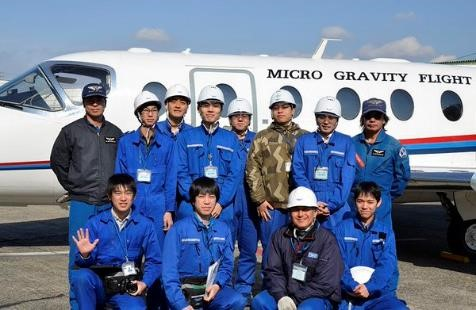
\includegraphics[width=.6\textwidth]{03/fig/3-9-3-1-13.jpg}
	\caption{航空機を用いた微小重力実験後の記念撮影}
	\label{fig3-9-3-1-13}
\end{figure}
	
\noindent \textbf{2016年12月12日 膜展開部単体振動試験:} 千葉産業支援技術研究所にて膜展開部EMの振動試験を実施した.ウェルリサーチ社(倉冨・日高)が計測を担当し,ペイロード担当としてサカセアドテック社の川端,衛星システム担当として東工大の坂本が立ち会った.振動試験前後で膜面の保持・展開機構の動作に違いが生じないことが検証できた.\vspace{2mm}

\noindent \textbf{2017年4月18日 EM伸展マスト付き展開実験:} 東工大古谷研にて,EM展開膜(平織膜+カプトンを用いたダミーデバイス)の4隅のブーム先端を天井から懸架する重力保証を行った状態での展開試験に成功した.長さ1mの伸展ブームも取り付け,さらに衛星バス部BBMも吊り下げて伸展カメラ部からの動画撮影も実施し,動画撮影にも成功した.これにより,主要なミッションの成立性を確認できた. 
\begin{figure}[H]
	\centering
	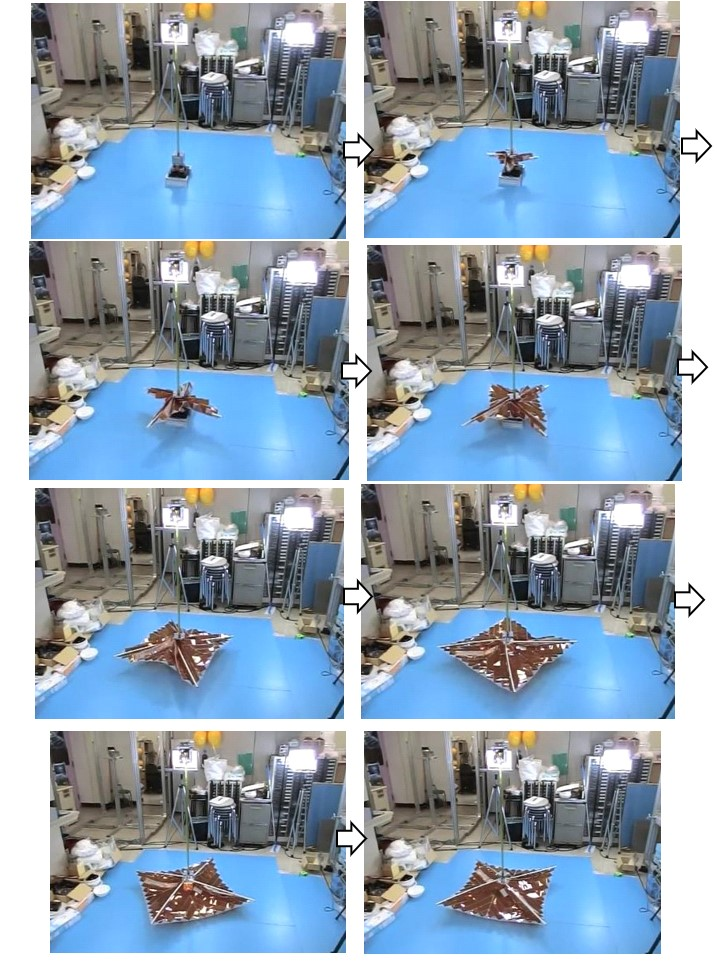
\includegraphics[width=.8\textwidth]{03/fig/3-9-3-1-5.jpg}
	\caption{伸展マスト付きEM膜の地上での展開実験}
	\label{fig3-9-3-1-5}
\end{figure}

\noindent \textbf{2017年10月16日~17日 真空槽内での展開実験:}日本大学宮崎研究室が有する真空槽を用いて,真空中での展開速度や展開オーバーシュート量の変化を観察した.宮崎研究室の支援のもと,古谷研究室が実験を主導した.EM膜を供試体として用いた.空気中での展開実験よりも大きなオーバーシュートが観察されたが,展開しきらないリスクよりは危険度が少ないと判断し,真空下での展開のオーバーシュートは許容する設計とした.
\begin{figure}[H]
	\centering
	\begin{tabular}{cc}
		\begin{minipage}{0.5\hsize}
			\begin{center}
				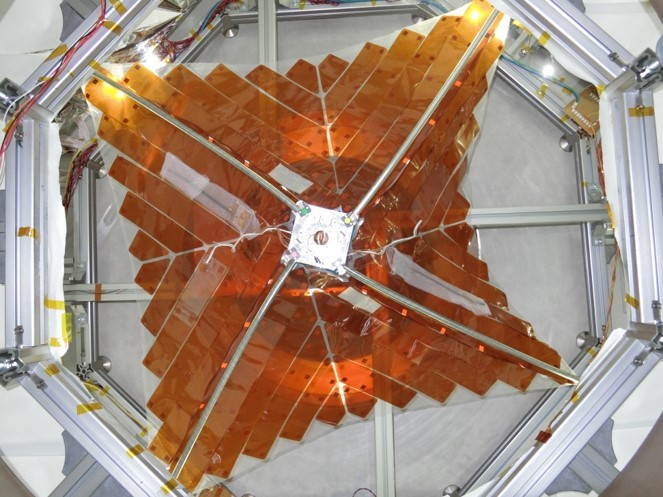
\includegraphics[width=1\textwidth]{03/fig/3-9-3-1-6.jpg}
			\end{center}
		\end{minipage}&
		\begin{minipage}{0.5\hsize}
			\begin{center}
				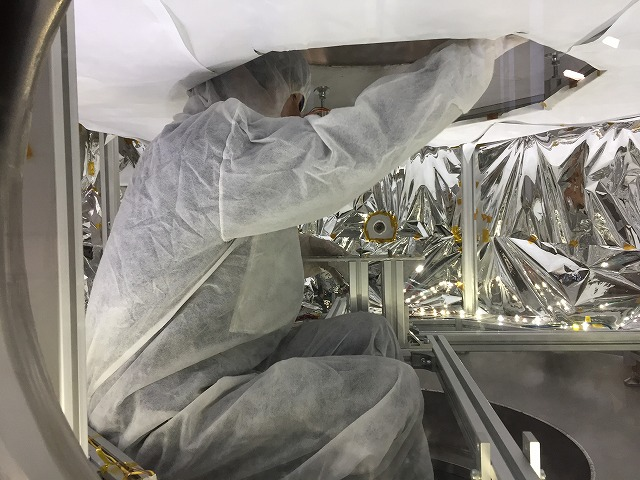
\includegraphics[width=1\textwidth]{03/fig/3-9-3-1-7.jpg}
			\end{center}
		\end{minipage}\\
		\begin{minipage}{0.5\hsize}
			\begin{center}
				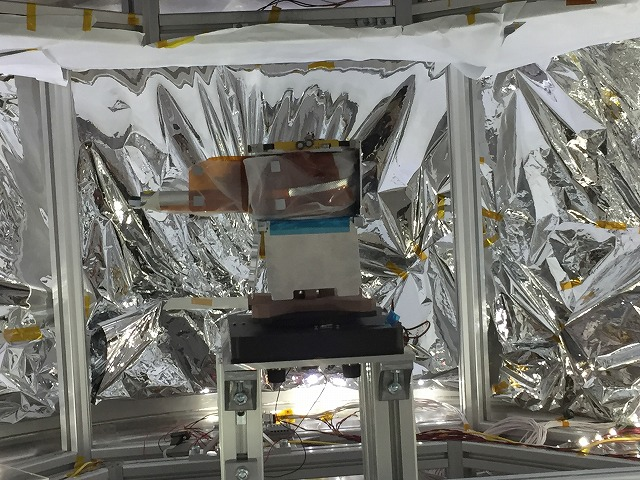
\includegraphics[width=1\textwidth]{03/fig/3-9-3-1-8.jpg}
			\end{center}
		\end{minipage}&
		\begin{minipage}{0.5\hsize}
			\begin{center}
				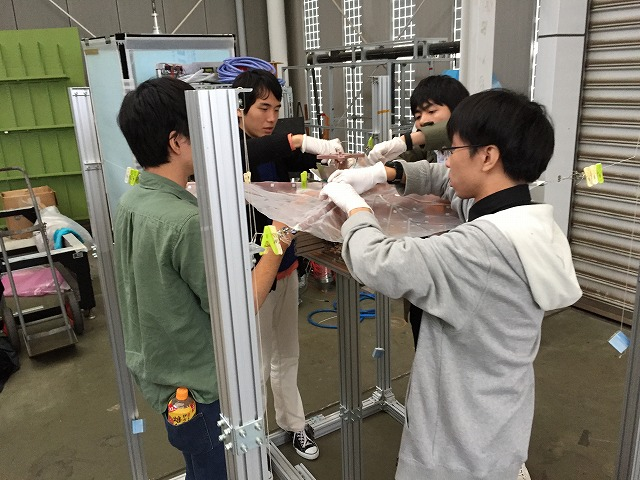
\includegraphics[width=1\textwidth]{03/fig/3-9-3-1-10.jpg}
			\end{center}
		\end{minipage}\\
			\begin{minipage}{0.5\hsize}
		\begin{center}
			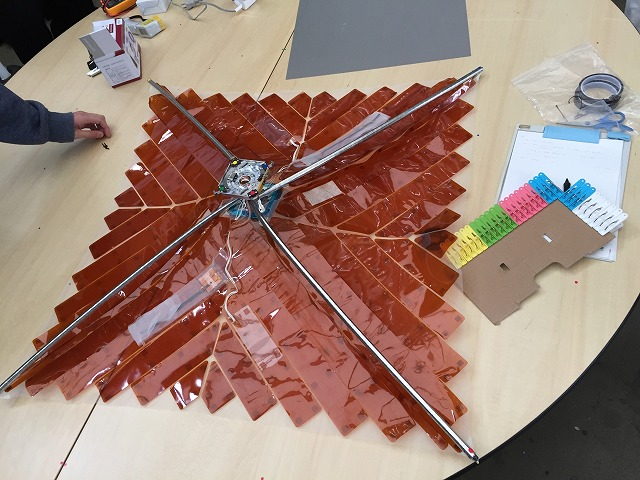
\includegraphics[width=1\textwidth]{03/fig/3-9-3-1-11.jpg}
		\end{center}
	\end{minipage}&
	\begin{minipage}{0.5\hsize}
		\begin{center}
			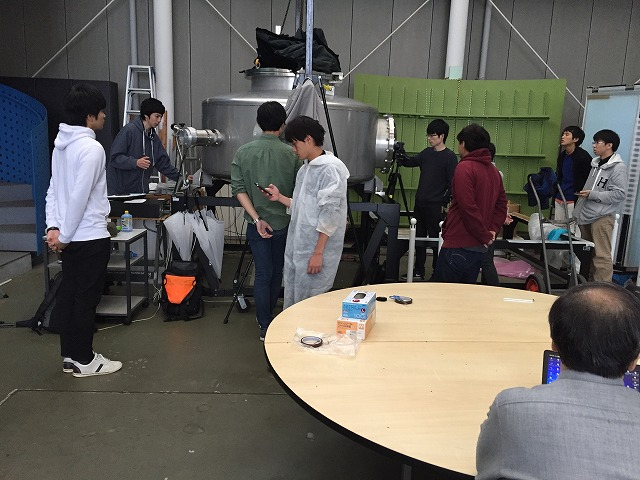
\includegraphics[width=1\textwidth]{03/fig/3-9-3-1-12.jpg}
		\end{center}
	\end{minipage}
	\end{tabular}
	\caption{日本大学におけるEM膜の真空層内での展開実験(2017年10月16~17日)}
	\label{fig3-9-3-1-6}
\end{figure}

\noindent \textbf{2017年11月15日 暗室内でのEM展開実験:} 古谷研の実験室の窓を暗幕で覆い,暗闇の中で伸展カメラ部のLED照射により展開動画が撮影できることを検証した.またこの実験後,EM振動試験,衝撃試験を実施した.\vspace{2mm}

\noindent \textbf{2018年1月19日 振動・衝撃試験後のEM展開実験:} 古谷研にて,健全な展開を検証した.
\begin{figure}[H]
	\centering
	\begin{tabular}{cc}
		\begin{minipage}{0.5\hsize}
			\begin{center}
				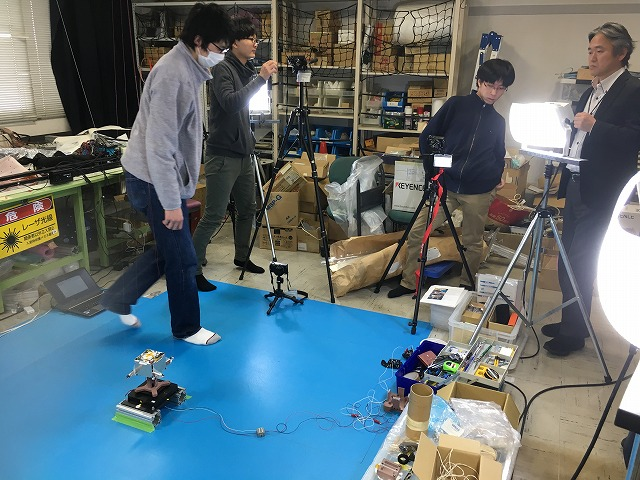
\includegraphics[width=1\textwidth]{03/fig/3-9-3-1-14.jpg}
			\end{center}
		\end{minipage}&
		\begin{minipage}{0.5\hsize}
			\begin{center}
				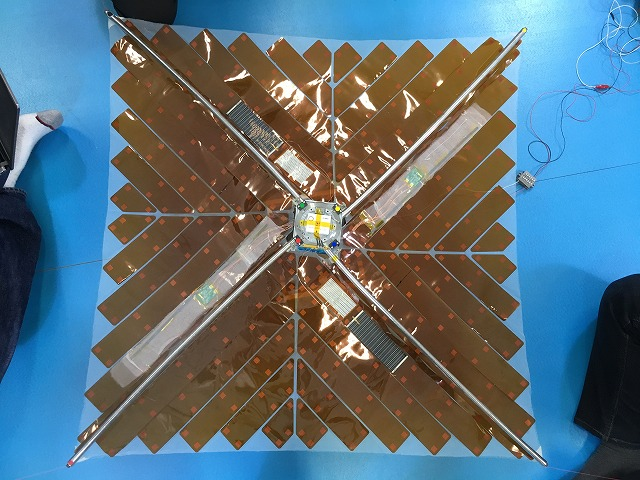
\includegraphics[width=1\textwidth]{03/fig/3-9-3-1-15.jpg}
			\end{center}
		\end{minipage}
	\end{tabular}
\caption{振動・衝撃試験後のEM展開実験(2018年1月19日)}
\label{fig3-9-3-1-14}
\end{figure}

\noindent \textbf{2018年4月11日 EM2膜収納・展開実験:} EMまではダミーデバイスとしてカプトン膜(75μm厚)を用いていたが,本体の発電量を減じる可能性があること,また厚く膜展開機構内に収納体積が収まらないこと,の2つの理由により,透明性の高いスペリオUT(50μm厚)によるダミーデバイスへと変更した.この膜を「EM2」膜と名付け,展開実験を行って健全な収納・展開を確認した.
\begin{figure}[H]
	\centering
	\begin{tabular}{cc}
		\begin{minipage}{0.5\hsize}
			\begin{center}
				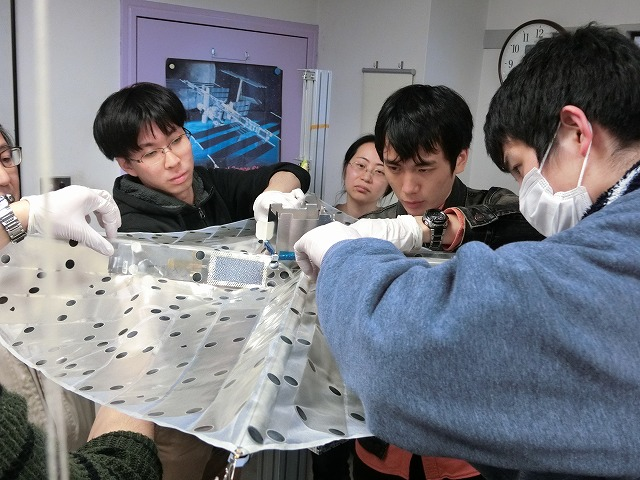
\includegraphics[width=1\textwidth]{03/fig/3-9-3-1-16.jpg}
			\end{center}
		\end{minipage}&
		\begin{minipage}{0.5\hsize}
			\begin{center}
				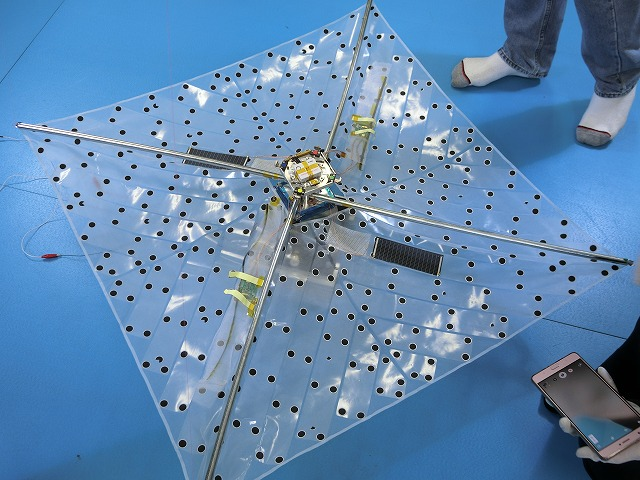
\includegraphics[width=1\textwidth]{03/fig/3-9-3-1-17.jpg}
			\end{center}
		\end{minipage}
	\end{tabular}
	\caption{EM2膜収納・展開実験(2018年4月11日)}
	\label{fig3-9-3-1-16}
\end{figure}

\noindent \textbf{2018年6月4日~6日 FM膜収納・展開実験:} FM膜が完成した.ブームの劣化を防ぐため,FMについては展開試験の回数を極力減らす選択をした.3日間で以下を実施した:
\noindent 状態確認/重量計測/薄膜太陽電池貼り付け/SMAアンテナ縫い付け/ハーネスの縫い付け/膜根元部-ブーム締結/重力補償用のラグ板取り付け/展開完了確認用マイクロスイッチ導通確認/溶断線抵抗計測/SMAアンテナ動作確認/展張状態での膜の垂れ下がり計測/展張状態での写真撮影/収納/ブーム先端位置の記録/カムに発生する張力のフォースゲージによる計測/テグス固定/収納状態の膜展開部の寸法計測(要求充足の確認)/展開実験/状態確認/再収納

EM2の展開挙動との違いは微小であり,機構の健全性を確認できた.\vspace{2mm}

\noindent \textbf{2018年6月29日 FM再収納:} 

膜の体積が大きく,ウォールで押さえつけていたが,ウォールの板およびヒンジの強度が十分でなく,FM膜収納後にヒンジが変形してしまい包絡域を逸脱する不具合があった.
このため,FM膜を一度取り出してヒンジを修理して再び取り付け,FM膜の膜上デバイスの量を減らして再収納する,という応急処置を施してフライトに臨んだ.
サカセアドテック社でヒンジを補修し,古谷研にて膜の再収納を行ったとき,(i) ブーム1本の根元にクラックが入っていることが発見された.これは補修せずにフライトすることとした.(ii) 1つウォールでねじりばねの先端が飛び出していた.折り返す補修をした.その上で再収納をしたが,やはりヒンジ部の変形が発生してしまっていた.

そこで,いま1度膜を開き,膜上アンテナのダミー基板を膜から取り外した.そしてこれまで以上にブームをつぶしながら,再度の収納を実施した.これにより,既定の寸法に収まる収納が実現できた.

最終的な膜展開部のテグスの固定は,2018年7月3日に古谷研・田村が担当した.

\subsubsection{テグス溶断機構(サカセアドテック・坂本)}

テグス溶断機構はサカセアドテックが設計・製作・各種試験を実施した.ボビン2つを使う,独自性の高い調整方法を採用している.下図に概要を示す.
\begin{figure}[H]
	\centering
		\centering
	\begin{tabular}{cc}
		\begin{minipage}{0.5\hsize}
			\begin{center}
				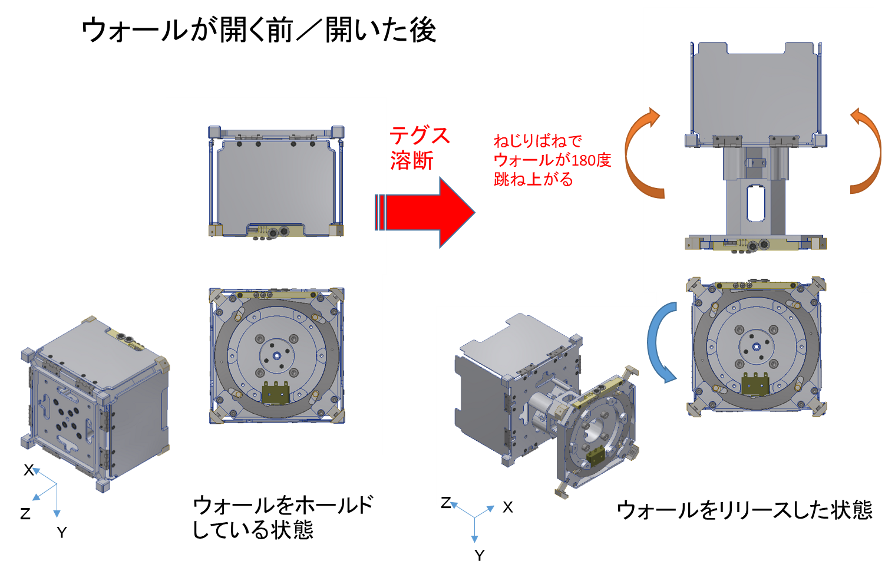
\includegraphics[width=1\textwidth]{03/fig/3-9-3-1-18.png}
			\end{center}
		\end{minipage}&
		\begin{minipage}{0.5\hsize}
			\begin{center}
				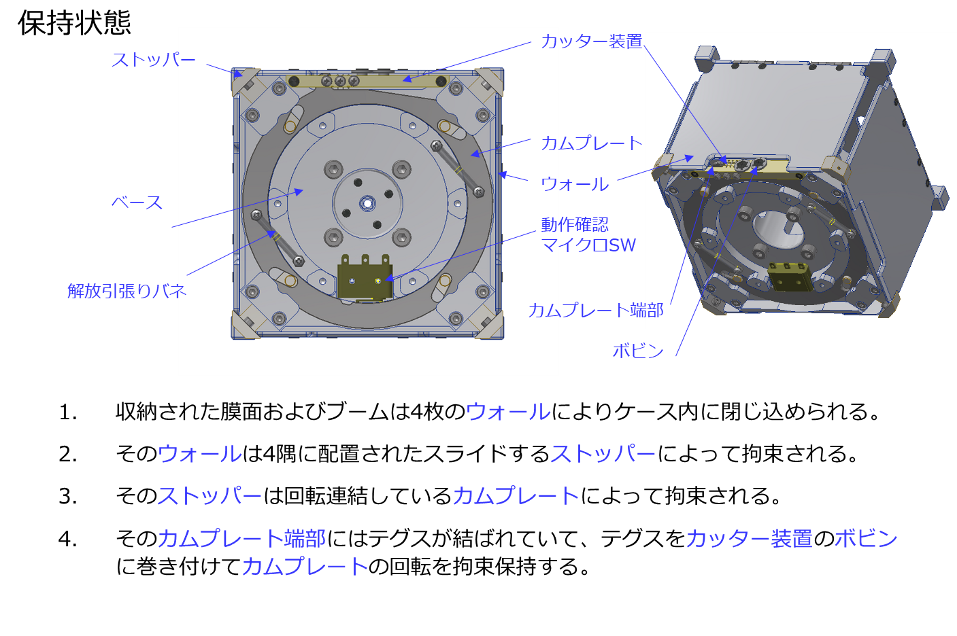
\includegraphics[width=1\textwidth]{03/fig/3-9-3-1-19.png}
			\end{center}
		\end{minipage}
	\end{tabular}
		\begin{tabular}{cc}
		\begin{minipage}{0.5\hsize}
			\begin{center}
				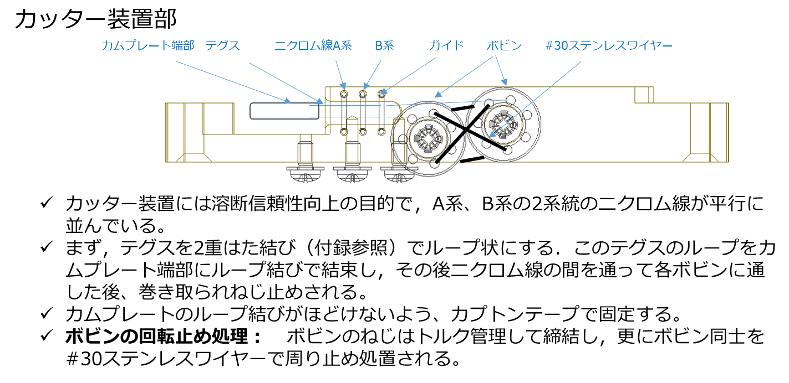
\includegraphics[width=1\textwidth]{03/fig/3-9-3-1-20.png}
			\end{center}
		\end{minipage}&
		\begin{minipage}{0.5\hsize}
			\begin{center}
				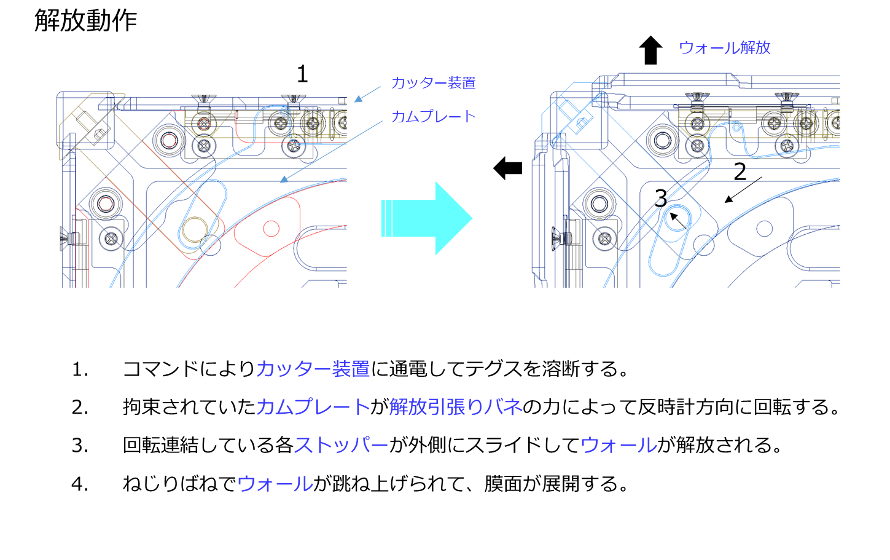
\includegraphics[width=1\textwidth]{03/fig/3-9-3-1-21.png}
			\end{center}
		\end{minipage}
	\end{tabular}
				\begin{tabular}{cc}
			\begin{minipage}{0.5\hsize}
				\begin{center}
					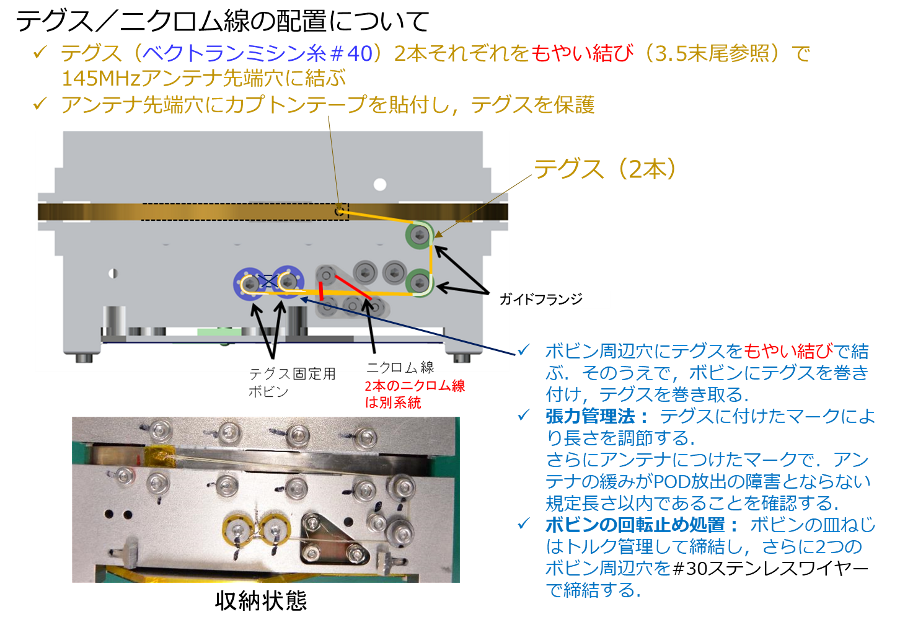
\includegraphics[width=.7\textwidth]{03/fig/3-9-3-1-22.png}
				\end{center}
			\end{minipage}&
			\begin{minipage}{0.5\hsize}
				\begin{center}
			  	   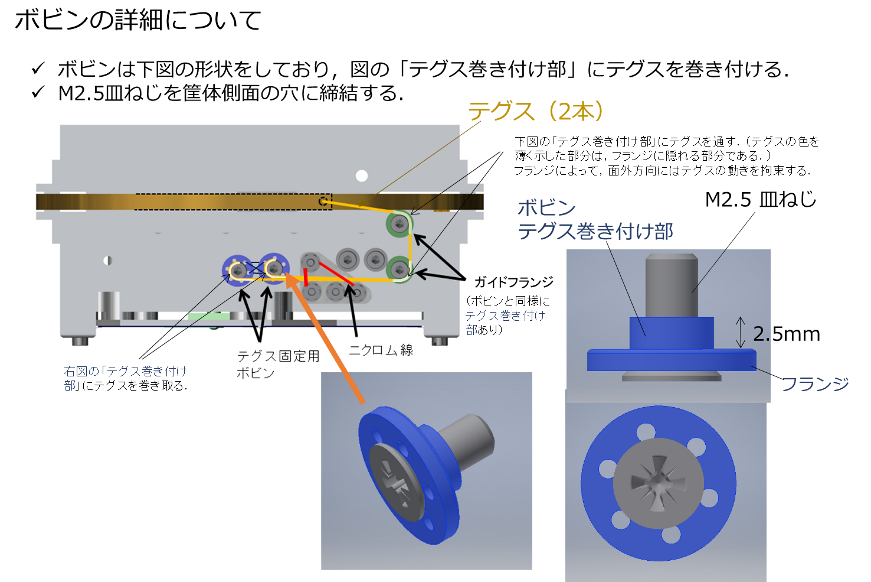
\includegraphics[width=.7\textwidth]{03/fig/3-9-3-1-23.png}
				\end{center}
			\end{minipage}
		\end{tabular}
		\caption{膜展開部の保持展開機構}
	\label{fig3-9-3-1-18}
\end{figure}

テグスの選定は,当初ダイニーマを使っていたが結び目が滑りやすいとサカセアドテックから指摘を受け,彼らが選定したベクトランを採用した.テグスの特性試験もサカセアドテックが実施した.
同じベクトランを,膜展開部だけでなく,伸展カメラ部,バス部(UHF/VHF展開アンテナ)のすべてで使用した.さらに膜展開部と同じボビンの調整機構をバス部(UHF/VHF展開アンテナ)でも採用した.

システム安全審査フェーズ2までは,誤展開がユニークハザードであったため,テグスの強度解析や特性試験結果報告,およびテグスを結ぶ詳細な手順書を作成した.しかし,システム安全審査フェース3で安全要求が緩和され,誤展開に関するユニークハザードレポートが廃止された.したがって,これらの文書はフェーズ3では提出しなかった.

詳細は下記文書を参照.特にJAXAのチェックリストは信頼性の高い機構を設計するうえで参考になった.
\begin{itemize}
	\item OP-S1-0085 テグス設計・試験報告書
	\item OP-S1-0030 テグス作業手順書
	\item OP-S1-0031 テグス作業報告書
	\item CSA-112040A 非金属ロックワイヤに関わる安全チェックリスト(JAXA文書): 上記OP-S1-0085末尾のチェックリストはこれを参照している.
\end{itemize}
